\subsection{Applications}
Toolpath\revise{}{s} with varying width is particularly meaningful for narrow parts, since there the negative effect of under- and overfill is more pronounced than in wide parts.
In extreme cases, thin features will not be filled at all.
Therefore, our framework, while working for wide parts as well, shows most of its potential for objects which contain thin parts.

\Cref{applications_overview} collectively shows the application of the proposed inward distributed scheme for various types of 3D model, including both thin parts (architectural models, casings, embossed text, gears and microstructures) and wide parts (\cref{applications_case}) and organic shapes (\cref{applications_statue})).

For architectural models and casings, preventing over- and underfill is expected to make them stronger. 
For embossed text, preventing underfill reduces the various holes in the top surfaces, which is detrimental to the visual quality of those top surfaces.
For gears and similar mechanical parts that are designed with finite element analysis, the less variation in extrusion widths is closer to the assumptions under fast analysis (e.g. using homogenization~\cite{Liu2016CAD}).

Of particular interest are microstructures that could be uniquely fabricated by 3D printing.
For example, topology optimized bone-like structures~\cite{wu2017infill} contain filaments of varying thickness that follow a varying stress direction (\cref{applications_bone}).
An angled Gyroid structure with uniform thickness also results in outline shapes with varying width (\cref{applications_gyroid}). 
These structures are accurately densely filled using our framework.
Another class of microstructures consists of parameterized patterns with varying thickness to achieve functional gradation.
\Cref{applications_hex} shows the contour-parallel toolpath with varying width of a hexagonal grid neatly switches between different bead counts over the volume, preventing the jagged moves a direction-parallel toolpath would create for such a case~\cite{bates2018compressive}.


\begin{figure*}
\centering
\setlength{\figwidth}{0.099\textwidth}
\setlength{\figheight}{0.099\textwidth}
\begin{subfigure}{\textwidth}\centering
\censorbox{
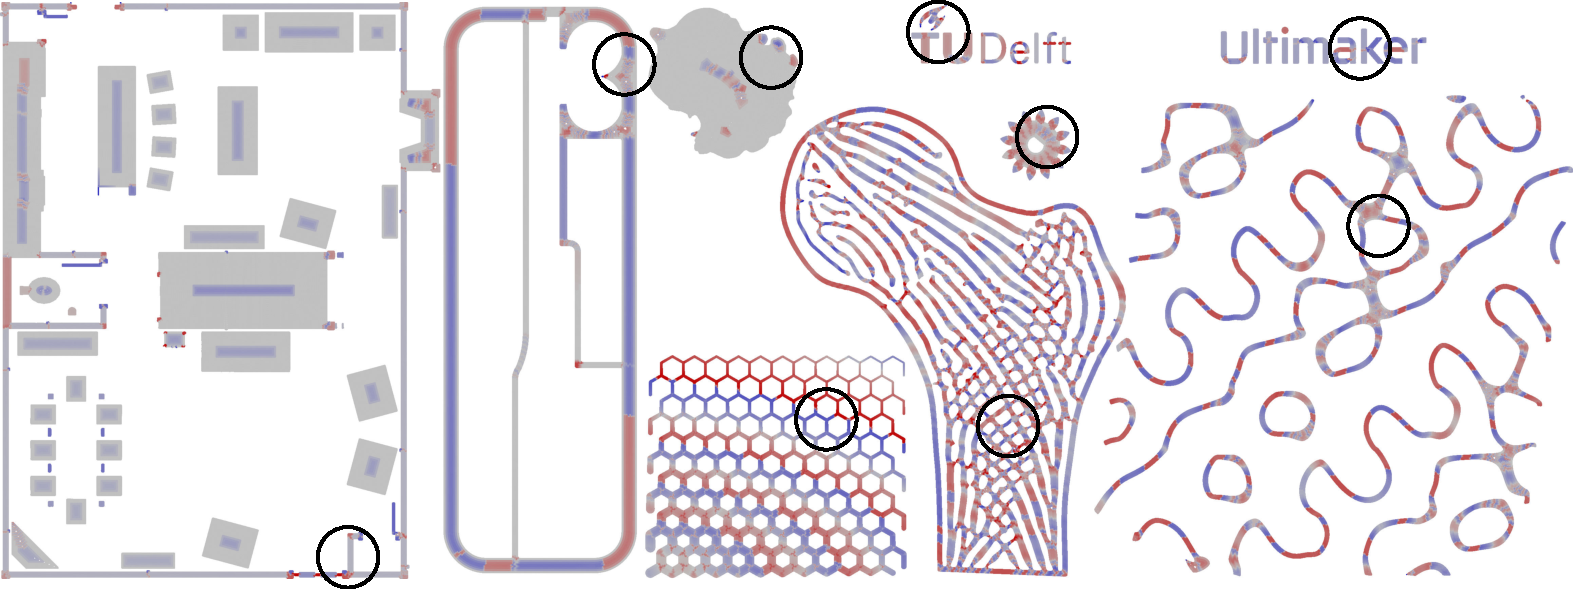
\includegraphics[width=\textwidth]{sources-applications-combined-small-dilated-circled.pdf}
}
%\caption{Overview}\label{applications_overview}
\end{subfigure}
\begin{subfigure}[t]{\figwidth}\centering
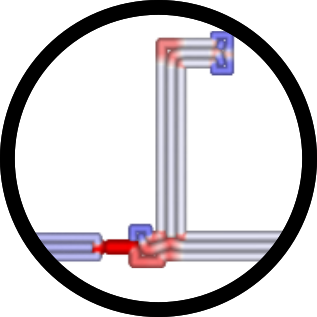
\includegraphics[height=\figheight]{sources-applications-house.png}
\caption{House}\label{applications_house}
\end{subfigure}
\begin{subfigure}[t]{\figwidth}\centering
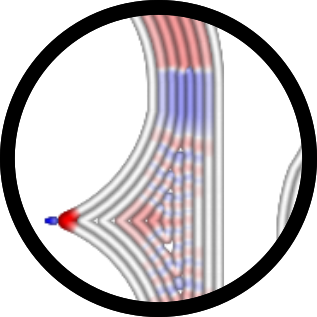
\includegraphics[height=\figheight]{sources-applications-pocket-operator-case.png}
\caption{Case}\label{applications_case}
\end{subfigure}
\begin{subfigure}[t]{\figwidth}\centering
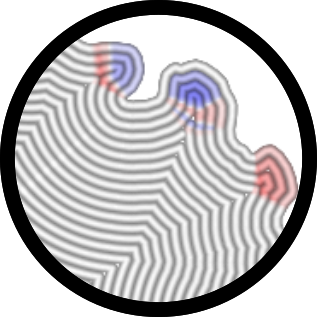
\includegraphics[height=\figheight]{sources-applications-david.png}
\caption{Statue}\label{applications_statue}
\end{subfigure}
\begin{subfigure}[t]{\figwidth}\centering
\censorbox{
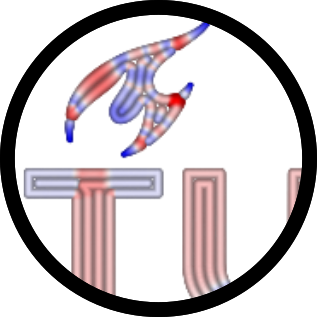
\includegraphics[height=\figheight]{sources-applications-tud-logo.png}
}
\caption{\censor{TUD}}\label{applications_tud}
\end{subfigure}
\begin{subfigure}[t]{\figwidth}\centering
\censorbox{

\includegraphics[height=\figheight]{sources-applications-ultimaker-logo.png}
}
\caption{\censor{UM}}\label{applications_um}
\end{subfigure}
\begin{subfigure}[t]{\figwidth}\centering
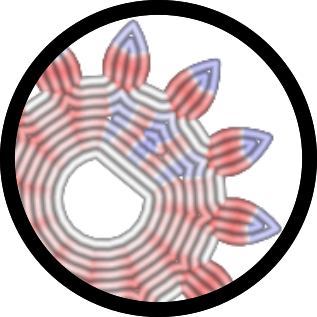
\includegraphics[height=\figheight]{sources-applications-pinion-gear-motor.png}
\caption{Gear}\label{applications_gear}
\end{subfigure}
\begin{subfigure}[t]{\figwidth}\centering
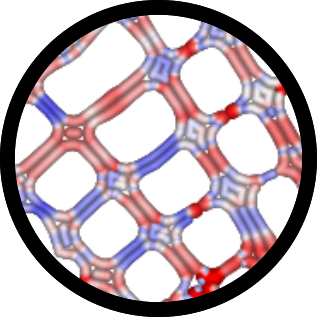
\includegraphics[height=\figheight]{sources-applications-topopt-bone.png}
\caption{Bone}\label{applications_bone}
\end{subfigure}
\begin{subfigure}[t]{\figwidth}\centering
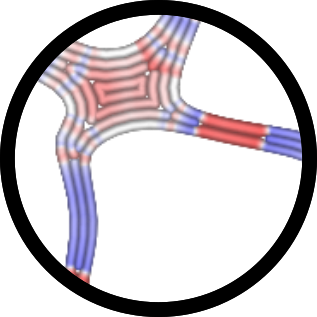
\includegraphics[height=\figheight]{sources-applications-gyroid.png}
\caption{Gyroid}\label{applications_gyroid}
\end{subfigure}
\begin{subfigure}[t]{\figwidth}\centering

\includegraphics[height=\figheight]{sources-applications-hex-grid.png}
\caption{Hex}\label{applications_hex}
\end{subfigure}
\begin{subfigure}[t]{.3\figwidth}
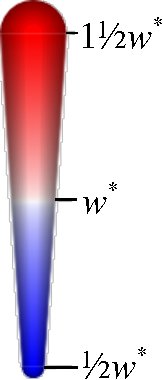
\includegraphics[height=\figheight]{sources-validation-widths-legend-small.pdf}
\end{subfigure}
\caption{
Visualization of the widths for the output toolpaths of the inward distributed beading scheme \revise{}{($N=3$) }applied to various example application objects.
From left to right and top to bottom: a house, a case for electronics, a statue, two common logos, a gear, a topologically optimized bone structure, a tilted homogeneous gyroid structure and a heterogeneous thickness hexagonal grid.
}
\label{applications_overview}
\end{figure*}




